\documentclass[../main]{subfiles}
\ifSubfilesClassLoaded{
    \dominitoc
    \tableofcontentsfile
}{}
\begin{document}
\chapter{Convergence de la relaxation}
\graphicspath{{./},{07-Relaxation/}}
\minitoc
Le processus de relaxation que nous proposons dans l'algorithme CxSOM est une méthode originale pour construire des connexions bidirectionnelles entre cartes. 
Deux cartes connectées de cette façon jouent alors un rôle symétrique. Dans cette section, nous évaluons expérimentalement la méthode de relaxation en tant que moyen de trouver une best matching unit (BMU).
La Best Matching Unit d'une carte de Kohonen correspond à la position où l'activité est maximale. 
Dans la situation d'une architecture de plusieurs cartes, ayant chacune un BMU, le vecteur de BMUs correspond à la positions ou chacune des activités est maximale. 
On est donc face à un problème de recherche de l'argument maximum d'activité dans lequel les activités dépendent les unes des autres. 
L'algorithme de relaxation proposé est une heuristique pour trouver ce point, s'il existe.

Pour considérer l'algorithme de relaxation comme une recherche de BMU, nous devons répondre aux questions suivantes:
\begin{itemize}
\item Est-ce que la méthode de relaxation converge ? 
\item Le point de convergence est il unique, c'est à dire relatif à l'état de la carte et non les conditions initiales ? 
\item L'activité au point d'arrivée de la relaxation traduit-elle 
\item Quels sont les paramètres à prendre en compte dans l'algorithme de relaxation ?
\end{itemize}

\section{Formalisation de l'algorithme de relaxation}

\subsection{Rappel du formalisme}

Le but de la relaxation est de chercher le vecteur de positions maximisant l'activité globale de chaque carte de l'architecture.
Cette activité étant positive, le problème revient à maximiser la somme des activités. Nous cherchons donc le vecteur de positions maximisant la somme des activités globales des cartes de l'architecture.


Notons $(\mathbf{\bmu})_\tau = (\bmu\m{0}_\tau,\cdots,\bmu\m{n}_\tau)$ la suite définie par l'évolution des BMUs des $N$ cartes d'une architecture lors de la relaxation.
La suite $(\mathbf{\bmu})_\tau$ est une suite définie par récurrence par $\mathbf{\bmu}_{\tau+1} = \mathbf{f}(\mathbf{\bmu}_\tau)$ avec $\mathbf{f} = (f\m{0},\cdots,f\m{n}) : [0,1]^N \rightarrow [0,1]^N$ une application non linéaire transformant l'espace des positions des BMUs; $\mathbf{f}$ ne dépend pas de $\tau$. 
L'algorithme de relaxation est alors une recherche de point fixe de la fonction $\mathbf{f}$.


Détaillons l'évolution de cette suite.
Pour clarifier les notations, définissons pour chaque carte~$i$ $\hat{p}\m{i}_\tau$, comme la position maximisant l'activité globale de la carte $i$:
\begin{equation}
\begin{gathered}
\hat{p}\m{i}_{\tau} = \argmax_{p\m{i}}(a_g\m{i}(p\m{i},\bmu\m{i_0}_\tau, \cdots \bmu\m{i_K}_\tau))\\
 i_0, \cdots i_K \: \text{indices des cartes nourrissant la carte $i$}.
\end{gathered}
\label{eq:pstar}
\end{equation}
$a_g\m{i}$ est une fonction des poids de la carte $\w\ext\m{i}, \w\cont\m{i}$ et de son entrée externe $\inpx\m{i}$. Lors du processus de relaxation, les poids et l'entrée restent fixes. Le calcul de $a_g$ ne dépend pas de $\tau$. Pour toute carte $i$, $\hat{p}\m{i}_{\tau}$ est donc seulement une fonction de $(\bmu\m{i_0}_\tau, \cdots \bmu\m{i_K}_\tau)$.
L'équation d'évolution s'écrit alors: 
\begin{equation}
\bmu\m{i}_{\tau+1} = 
\begin{cases}
\bmu\m{i}_{\tau} + sgn(\hat{p}\m{i}_{\tau} - \bmu\m{i}_{\tau}) \times \delta \; & \text{si $\hat{p}\m{i}_{\tau} - \bmu\m{i}_{\tau} > \delta$ } \\
\hat{p}\m{i}_{\tau} \; \text{sinon}	
\end{cases}
\label{eq:evolution}
\end{equation}

En posant $f\m{i}$ la partie droite de l'équation \ref{eq:evolution}, on peut donc écrire: 
\begin{equation}
\bmu\m{i}_{\tau +1} = f\m{i}(\bmu\m{0}_\tau,\cdots,\bmu\m{n}_\tau)
\label{eq:fonction}
\end{equation}
Soit, pour l'ensemble des composantes: 
\begin{equation}
\mathbf{\bmu}_{\tau+1} = \mathbf{f}(\mathbf{\bmu}_\tau)
\end{equation}

La relaxation se traduit ainsi par une recherche de point fixe de la suite $(\mathbf{\bmu})_{\tau}$, soit une position $\mathbf{\bmu}$ telle que:
\begin{equation}
\mathbf{\bmu} = \mathbf{f}(\mathbf{\bmu})
\label{eq:suite}
\end{equation}

Si $f$ admet un point fixe, alors ce point fixe est aussi un point fixe pour la suite $(\mathbf{\bmu})_\tau$. Cependant, rien ne garantit que ce point fixe existe, ni que la suite converge.
Expérimentalement, il semble que si $\mathbf{f}$ admet un unique point fixe et que les poids $\w$ présentent une continuité, alors $(\mathbf{\bmu})_{\tau}$ converge vers ce point fixe. 

L'évolution de la suite $(\mathbf{\bmu})_{\tau}$ dépend de son initialisation.
L'état initial $(\bmu\m{0}_0, \cdots , \bmu\m{n}_0)$ est défini dans CxSOM par: 
\begin{equation}
\begin{cases}
\bmu\m{0}_0 = \argmax_{p\m{0}} a_e(p\m{0},\inpx\m{0})\\
\cdots \\
\bmu\m{n}_0 = \argmax_{p\m{n}} a_e(p\m{n},\inpx\m{n})\\
\end{cases}
\label{eq:init}
\end{equation}


Dans les sections suivantes, nous utiliserons des entrées formant un cercle en une dimension dans un espace en deux ou trois dimensions. Les entrées d'une carte correspondent à la coordonnée des points sur un des axes $X$,$Y$ et $Z$ en trois dimensions.
Les architectures étudiées sont des cartes 1D, et 2D lorsque cela est précisé. Les cartes sont connectées réciproquement, comme indiqué en figure \ref{fig:archis}.
Nous chercherons, sur ce jeu de données, à vérifier si la relaxation converge, et comment les paramètres et l'initialisation de la relaxation influencent les trajectoires et la convergence.
\begin{figure}
\centering
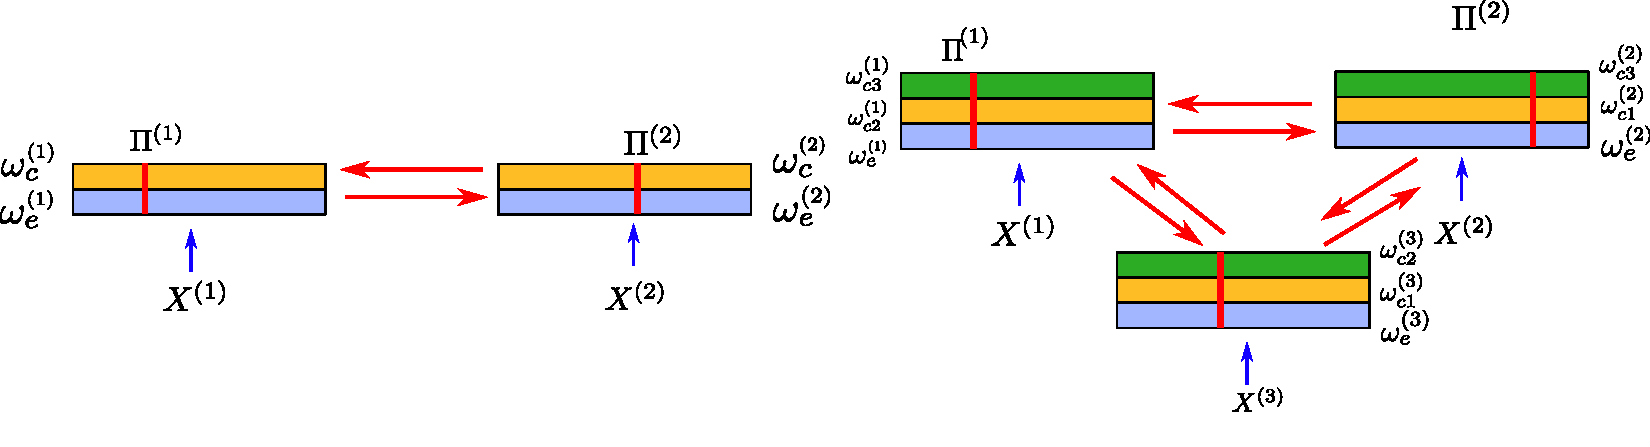
\includegraphics[width=\textwidth]{archis}
\caption{Architectures de deux et trois cartes utilisées dans cette section. Les cartes peuvent être en une ou deux dimensions. Dans le cas de cartes en deux dimensions, la position du BMU $\bmu$ est alors un vecteur 2D.}
\label{fig:archis}
\end{figure}

\subsection{Quelles propriétés attend-on d'une Best Matching Unit ?}

La notion de Best Matching Unit est définie au sein de l'algorithme d'apprentissage d'une carte de Kohonen, comme l'unité possédant l'activité maximale pour une entrée fixée. Cette activité dépend de l'entrée présentée et des poids de la carte, mais peut aussi dépendre d'autres facteurs pour d'autres modèles de carte, tels que l'état de la carte au temps précédent pour les cartes récurrentes, ou dans notre cas les positions des BMU des cartes adjacentes.
Dans le modèle classique de carte auto-organisatrice, nous pouvons dégager les propriétés suivantes concernant la BMU:
\begin{itemize}
	\item La BMU est seulement relative à l'état de la carte (activités) et sa ou ses entrées. Notons qu'en règle générale, ce BMU est unique. Cependant, plusieurs poids peuvent être égaux dans une carte et correspondre à l'activité maximale. Ce cas est de probabilité nulle pour un espace d'entrée continu. 
	Notons donc que l'existence de plusieurs positions correspondant au maximum de l'activité est un cas dégénéré à prendre en compte, mais peu atteint en pratique.
	\item La recherche du BMU est déterministe. Encore une fois, dans le cas de plusieurs BMU possibles, ce n'est plus vrai, mais la recherche du BMU est alors limitée à un nombre réduit de possibilités.
	\item Le poids du BMU est une approximation de la valeur d'entrée.
\end{itemize}
Dans l'algorithme CxSOM, la recherche du BMU est réalisée par une méthode dynamique de relaxation. 
Pour observer les mêmes propriétés sur la recherche classique par activité dans une carte simple et la recherche par relaxation, il est nécessaire que:
\begin{itemize}
	\item La recherche du BMU converge. En effet, s'il n'existe pas de point de convergence, nous ne pouvons pas définir un unique BMU pour la carte. 
	\item La valeur trouvée à l'issue de la relaxation ne dépend pas des conditions de l'expérience, à savoir les conditions initiales de la relaxation. De cette façon, un BMU est relatif à l'état de la carte, le processus de relaxation est déterministe.
	\item Le poids externe du BMU approxime l'entrée. Les calculs d'activités s'appuient sur une distance euclidienne entre le poids du BMU et l'entrée. Ce poids devrait donc être une approximation correcte de la valeur d'entrée.
\end{itemize}

Nous chercherons donc à évaluer si ces conditions sont remplies pour l'algorithme CxSOM. 
Notons que dans l'algorithme CxSOM, les BMUs sont initialisés à la position du maximum de l'activité externe dans chaque carte. 
Nous effectuerons l'analyse de la relaxation pour des conditions initiales quelconques, mais il est important de noter que ce choix d'initialisation permettra d'éviter des cas de non convergence.

Nous montrerons expérimentalement qu'il n'existe pas toujours un unique point fixe, notamment lorsque les poids sont aléatoirement répartis au début de l'apprentissage, ce qui entraîne alors une non-convergence de la relaxation. 
Cependant, nous observons que ces cas de non-convergence n'influencent pas l'apprentissage des cartes, ce qui est notamment permis par l'initialisation des positions au maximum de l'entrée externe.
Nous observera expérimentalement qu'à la fin de l'apprentissage, la disposition des poids permet l'existence d'un unique point fixe qui est indépendant de l'initialisation des valeurs de $\bmu\m {i}_{\tau}$.

Ce chapitre est une étude empirique de ce processus de relaxation, réalisée sur des dispositions d'entrées particulières: un cercle en deux et trois dimensions.
La démarche expérimentale est la suivante:
Nous étudierons d'abord l'influence de l'entrée contextuelle sur la valeur du BMU. Cet étude nous permet d'avoir des éléments de preuve de convergence.
Nous étudierons ensuite expérimentalement l'unicité du point fixe en fonction des conditions initiales de la relaxation.
Enfin, nous verrons comment le choix du pas de relaxation $\Delta$ influence la relaxation.

\section{Etude expérimentale de la convergence de la relaxation}

La méthode de relaxation cherche un point de convergence des BMU $\bmu\m{i}$ de l'architecture. Nous avons réalisé 1000 itérations de test, à poids figés, à différents temps d'apprentissage, et comptons le nombre de pas nécessaires à la convergence de la relaxation. L'algorithme utilisé pour la relaxation s'arrête automatiquement si la relaxation dépasse $\tau_{max}= 1000$ itérations; on considérera que la relaxation n'a pas atteint un point de convergence si la relaxation atteint ces $\tau_{max}$ itérations.

Plusieurs situations peuvent se traduire par une non-convergence de la relaxation:
\begin{itemize}
\item La relaxation évolue vers un point de convergence, mais trop lentement pour y arriver en moins de 1000 itérations
\item La relaxation évolue vers un cycle limite composé d'un nombre limité d'unités étant alternativement best matching units
\item La relaxation évolue sans répétition de motifs dans les cartes : évolution chaotique.
\end{itemize}
Le premier cas est évité car la limite de 1000 itérations est assez grande par rapport à la taille de la carte, les cartes étant de taille 500. Le pas d'évolution de la relaxation est d'une dizaine d'unités. La convergence, si elle existe, est donc rapide. Les cas de non-convergence concernent alors la deuxième et la troisième situation.
Nous observerons plus précisément les trajectoires dans la section suivante; on s'intéresse ici seulement à la question de la convergence.
L'étude de la convergence sera réalisée dans des architectures de 2 et 3 cartes, pour des cartes une dimension et deux dimensions.

La figure \ref{fig:conv_evolution} présente l'évolution du taux de convergence au cours de l'apprentissage d'une architecture de 2 cartes et 3 cartes. La figure \ref{fig:conv_evolution2D} trace  cette évolution dans le cas de cartes 2D. Pour tracer cette évolution, on effectue des étapes de tests à intervalles réguliers au cours de l'apprentissage, pendant lesquelles les poids ne sont pas mis à jour. Ces tests sont réalisés sur 1000 entrées externes $\inpx\m{1} = X, \inpx\m{2}=Y$ (et $\inpx\m{3}=Z$ pour trois cartes), prises aléatoirement dans l'espace d'entrée. 
On compte, pour chaque échantillon de test, le nombre de pas nécessaire à la relaxation. 
Si ce nombre est égal à $\tau_{max}$, on considère que la relaxation n'a pas convergé. 
On trace alors, en haut, le pourcentage d'échantillons de test pour lesquel la relaxation converge. En bas, on trace le nombre moyen de pas de relaxation nécessaires à la convergence.
Dans chaque cas, on répètera 10 fois l'apprentissage complet et les tests, sur le même espace d'entrée mais des éléments différents. Les tracés des figures \ref{fig:conv_evolution} et \ref{fig:conv_evolution2D} sont la moyenne et l'écart type des valeurs obtenues sur ces 10 répétitions.

Au début de l'apprentissage, lorsque les poids sont initialisés aléatoirement, la relaxation atteint rarement un point de convergence. Lorsque les cartes se déplient, la relaxation évolue vers un point de convergence dans plus de $90 \%$ des cas. Cette évolution est similaire pour des architecture de deux et trois cartes. Les expériences avec des cartes en deux dimensions présentent la même évolution. Le taux de convergence en fin d'apprentissage est plutot situé entre $80 \%$ et $90 \%$.
 
\begin{figure}
\centering
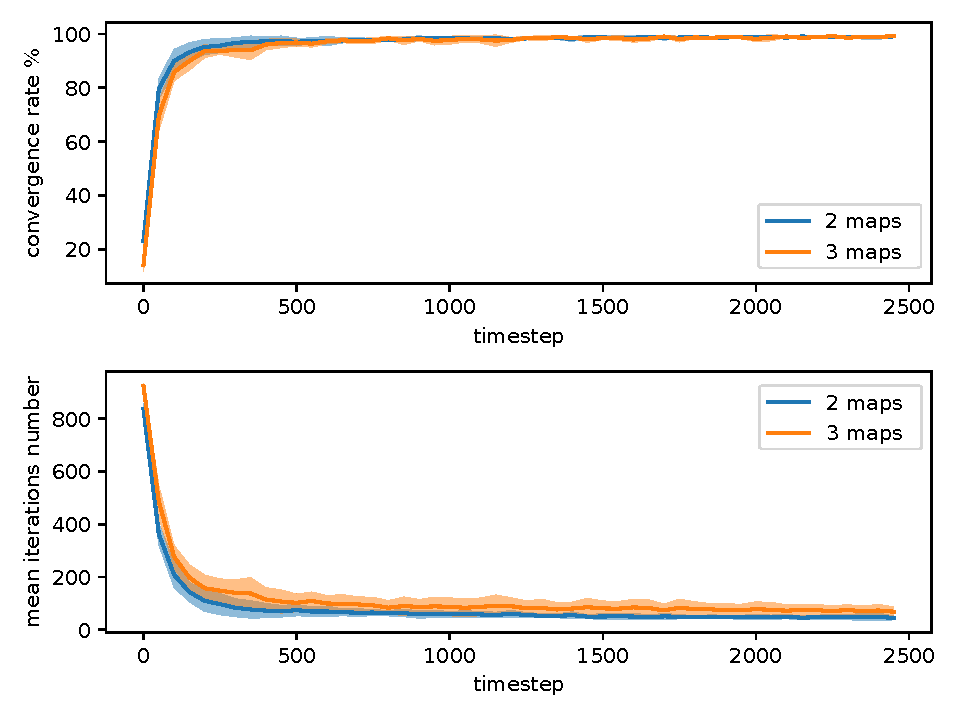
\includegraphics[width=0.7\textwidth]{1D_conv_evolution_total.pdf}
\caption{En haut: évolution de la moyenne et l'écart-type du taux de convergence lors de la relaxation au cours de l'apprentissage sur deux et trois cartes 1D. En bas: évolution du nombre moyen de pas nécessaires à la convergence de la relaxation.
Chaque point est calculé sur un échantillon de 1000 relaxations au temps t, évaluées sur des entrées différentes prises aléatoirement sur le cercle. La moyenne et l'écart-type sont réalisés sur 10 apprentissages séparés.}
\label{fig:conv_evolution}
\end{figure}


\begin{figure}
\centering
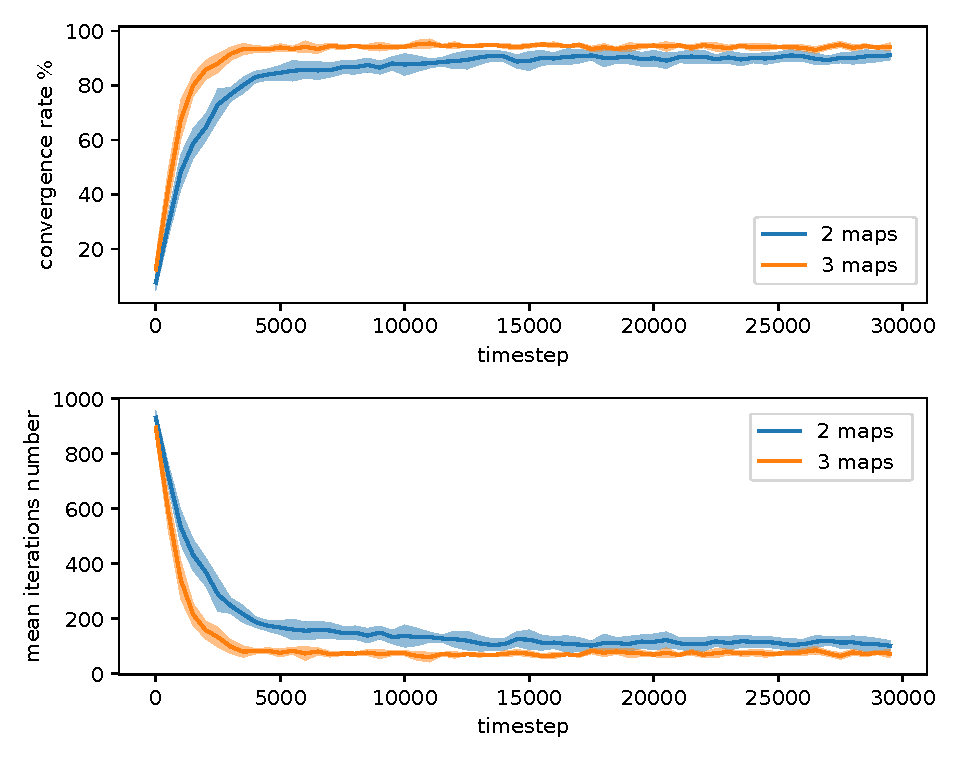
\includegraphics[width=0.7\textwidth]{2D_conv_evolution_total.pdf}
\caption{En haut: évolution de la moyenne et écart type taux de convergence lors de la relaxation au cours de l'apprentissage sur deux et trois cartes 2D. Chaque point est calculé sur un échantillon de 1000 relaxations au temps t, évaluées sur des entrées différentes prises aléatoirement sur le cercle. Les moyennes et écart types sont calculés sur 10 apprentissages séparés.}
\label{fig:conv_evolution2D}
\end{figure}
\section{Analyse paramétrique de la relaxation}

\subsection{Influence de l'initialisation \label{sec:pf}}

Nous étudions dans cette partie l'évolution de processus de relaxation lancés sur les mêmes poids, pour une entrée externe fixée, mais avec $\mathbf{\bmu}_0$ intialisés à des valeurs aléatoires dans chaque carte.
En figure \ref{fig:diff_relax_t1_notraj} et \ref{fig:diff_relax_notraj}, nous représentons les valeurs $\lvert \hat{p}\m{1} - p\m{1} \rvert$ et $\lvert \hat{p}\m{2} - p\m{2}\rvert$ en fonction de $p\m{1},p\m{2} \in [0,1]$, au début et fin de l'apprenitssage. On rappelle que $\hat{p}\m{1}$ dépend de $p\m{2}$, et inversement.
Le point fixe, s'il existe, est alors à une position $p\m{1},p\m{2}$ vérifiant:
\begin{equation*}
\begin{cases}
\hat{p}\m{1} = p\m{1}\\
\hat{p}\m{2} = p\m{2}\\
\end{cases}
\end{equation*}

On effectue 200 trajectoires de relaxation, initialisées à $\bmu\m{1}_0,\bmu\m{2}_0$ différents. Leurs valeurs finales sont représentées par un point noir en figures \ref{fig:diff_relax_t1_notraj} et \ref{fig:diff_relax_notraj}. 
Au début de l'apprentissage, la fonction de relaxation présente plusieurs points d'attraction, représentés par les points noirs en figure \ref{fig:diff_relax_t1_notraj}. Cette non-convergence semble s'expliquer par les valeurs des différences $\lvert \hat{p}\m{1} - p\m{1} \rvert$ et $\lvert \hat{p}\m{2} - p\m{2}\rvert$. Les zones en violet sur chaque figure représentent les positions où ces différences sont nulles, sur la carte 1 et 2. Un point fixe se trouve sur une position telle que les différences sont nulles dans les deux figures. Une telle position semble exister en figure \ref{fig:diff_relax_t1_notraj}, mais peu de trajectoires de relaxation y aboutissent. La figure \ref{fig:champ_0} représente le déplacement à effectuer de $(\bmu\m{1},\bmu\m{2})$ lors de la relaxation en fonction de la position courante. Les trajectoires des relaxations y sont également représentées. Le champ de déplacement ne semble pas permettre de trouver un point de convergence.
A la fin de l'apprentissage, ce qui est représenté en figure \ref{fig:diff_relax_notraj}, un point fixe semble exister. Ce point correspond à la position où les deux différences $\lvert \hat{p}\m{1} - p\m{1} \rvert$ et $\lvert \hat{p}\m{2} - p\m{2}\rvert$ sont nulles. Les 200 trajectoires mènent au même point, il semble donc être un point de convergence commun à toutes les initialisations pour la relaxation. La figure \ref{fig:champ_9999} présente le champ de déplacement des BMUs en fonction de la position courante. Les trajectoires suivent les zones où l'une ou l'autre des différences est nulle, pour mener à la position stable. 


\begin{figure}
\begin{minipage}{0.5\textwidth}
\centering
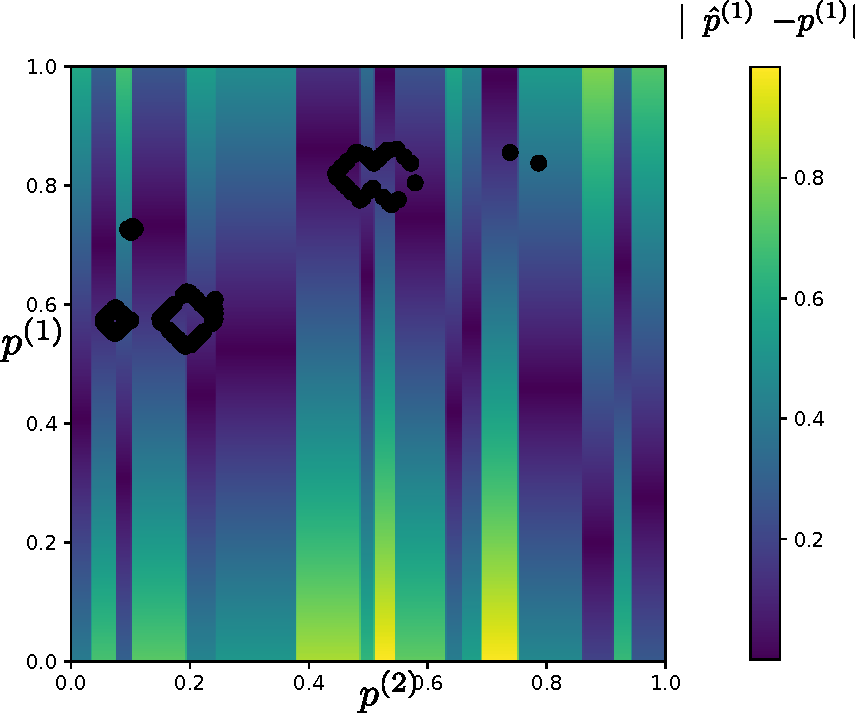
\includegraphics[width=\textwidth]{champ_X_006_t1_notraj.pdf}
\end{minipage}
\begin{minipage}{0.5\textwidth}
\centering
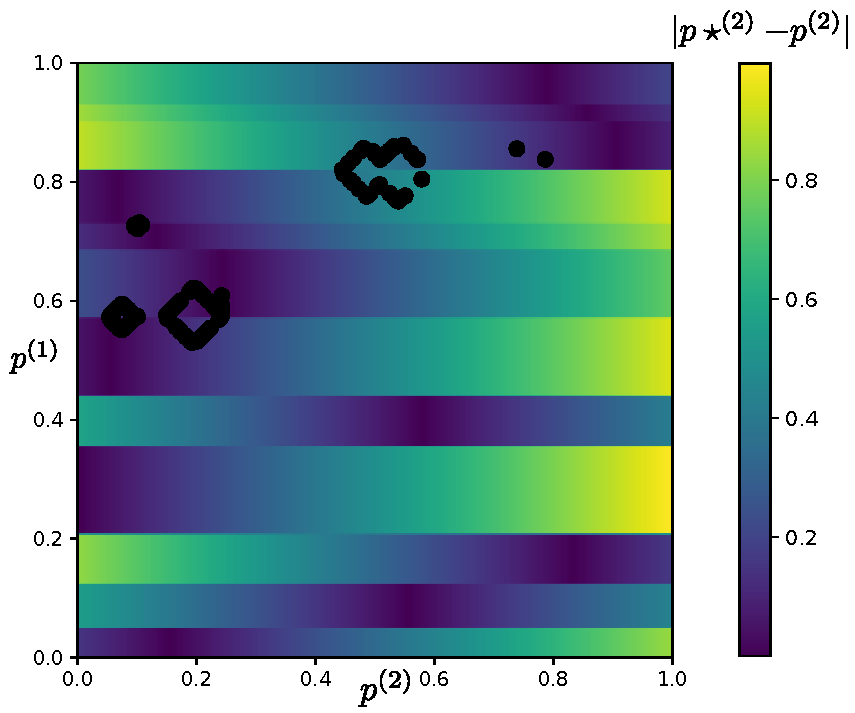
\includegraphics[width=\textwidth]{champ_Y_006_t1_notraj.pdf}
\end{minipage}
\caption{Valeur de ${\hat{p}}\m{1} - p\m{1}$, resp. ${\hat{p}}\m{2} - p\m{2}$ à $t=0$ ,lorsque les poids sont encore aléatoiremement disposés dans chaque carte.
 ${\hat{p}}\m{1}$ ne dépend que de $p\m{2}$ : on peut donc tracer cette valeur selon deux dimensions pour chaque carte. Les zones où cette valeur est nulle sont en violet sur le graphique. Les points fixes, s'il existent, sont aux positions de différence nulle pour $M\m{1}$ et $M\m{2}$. Les points noirs représentent les points de convergence pour 200 trajectoires de relaxation, lancées pour différents $\bmu_0\m{1}, \bmu_0\m{2}$.}
 
\label{fig:diff_relax_t1_notraj}
\end{figure}

\begin{figure}
\begin{minipage}{0.5\textwidth}
\centering
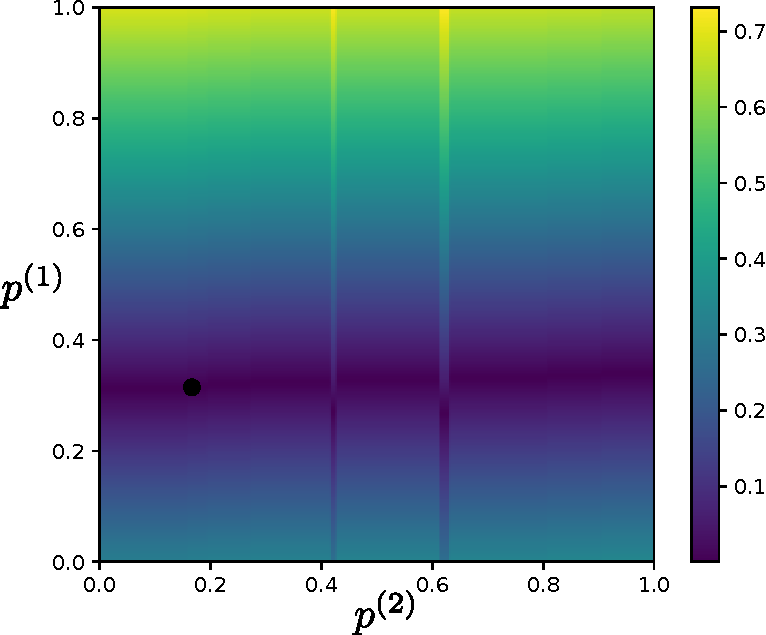
\includegraphics[width=\textwidth]{champ_X_006_notraj.pdf}
\end{minipage}
\begin{minipage}{0.5\textwidth}
\centering
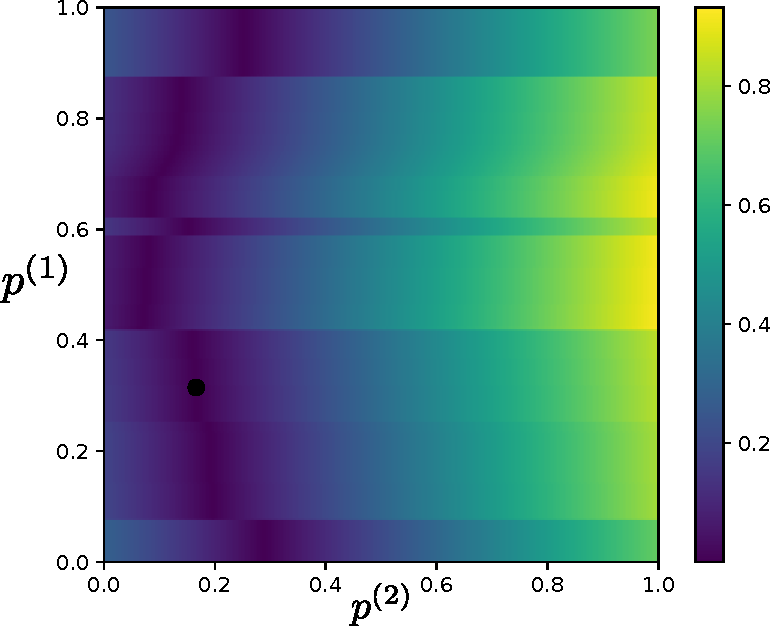
\includegraphics[width=\textwidth]{champ_Y_006_notraj.pdf}
\end{minipage}
\caption{Valeur de ${\hat{p}}\m{1} - p\m{1}$, resp. ${\hat{p}}\m{2} - p\m{2}$, lorsque les cartes sont organisées telles qu'en figure \ref{fig:w006}. ${\hat{p}}\m{1}$ ne dépend que de $p\m{2}$ : on peut donc tracer cette valeur selon deux dimensions pour chaque carte. Les zones où cette valeur est nulle sont en violet sur le graphique. Les points fixes, s'il existent, sont aux positions de différence nulle pour $M\m{1}$ et $M\m{2}$. Les points noirs représentent les points d'arrivée de la relaxation pour 50 trajectoires de relaxation, lancées pour différents $\bmu_0\m{1}, \bmu_0\m{2}$. La relaxation semble présenter un point de convergence, qui se situe sur un point fixe de la fonction de relaxation.}
\label{fig:diff_relax_notraj}
\end{figure}

\begin{figure}
\centering
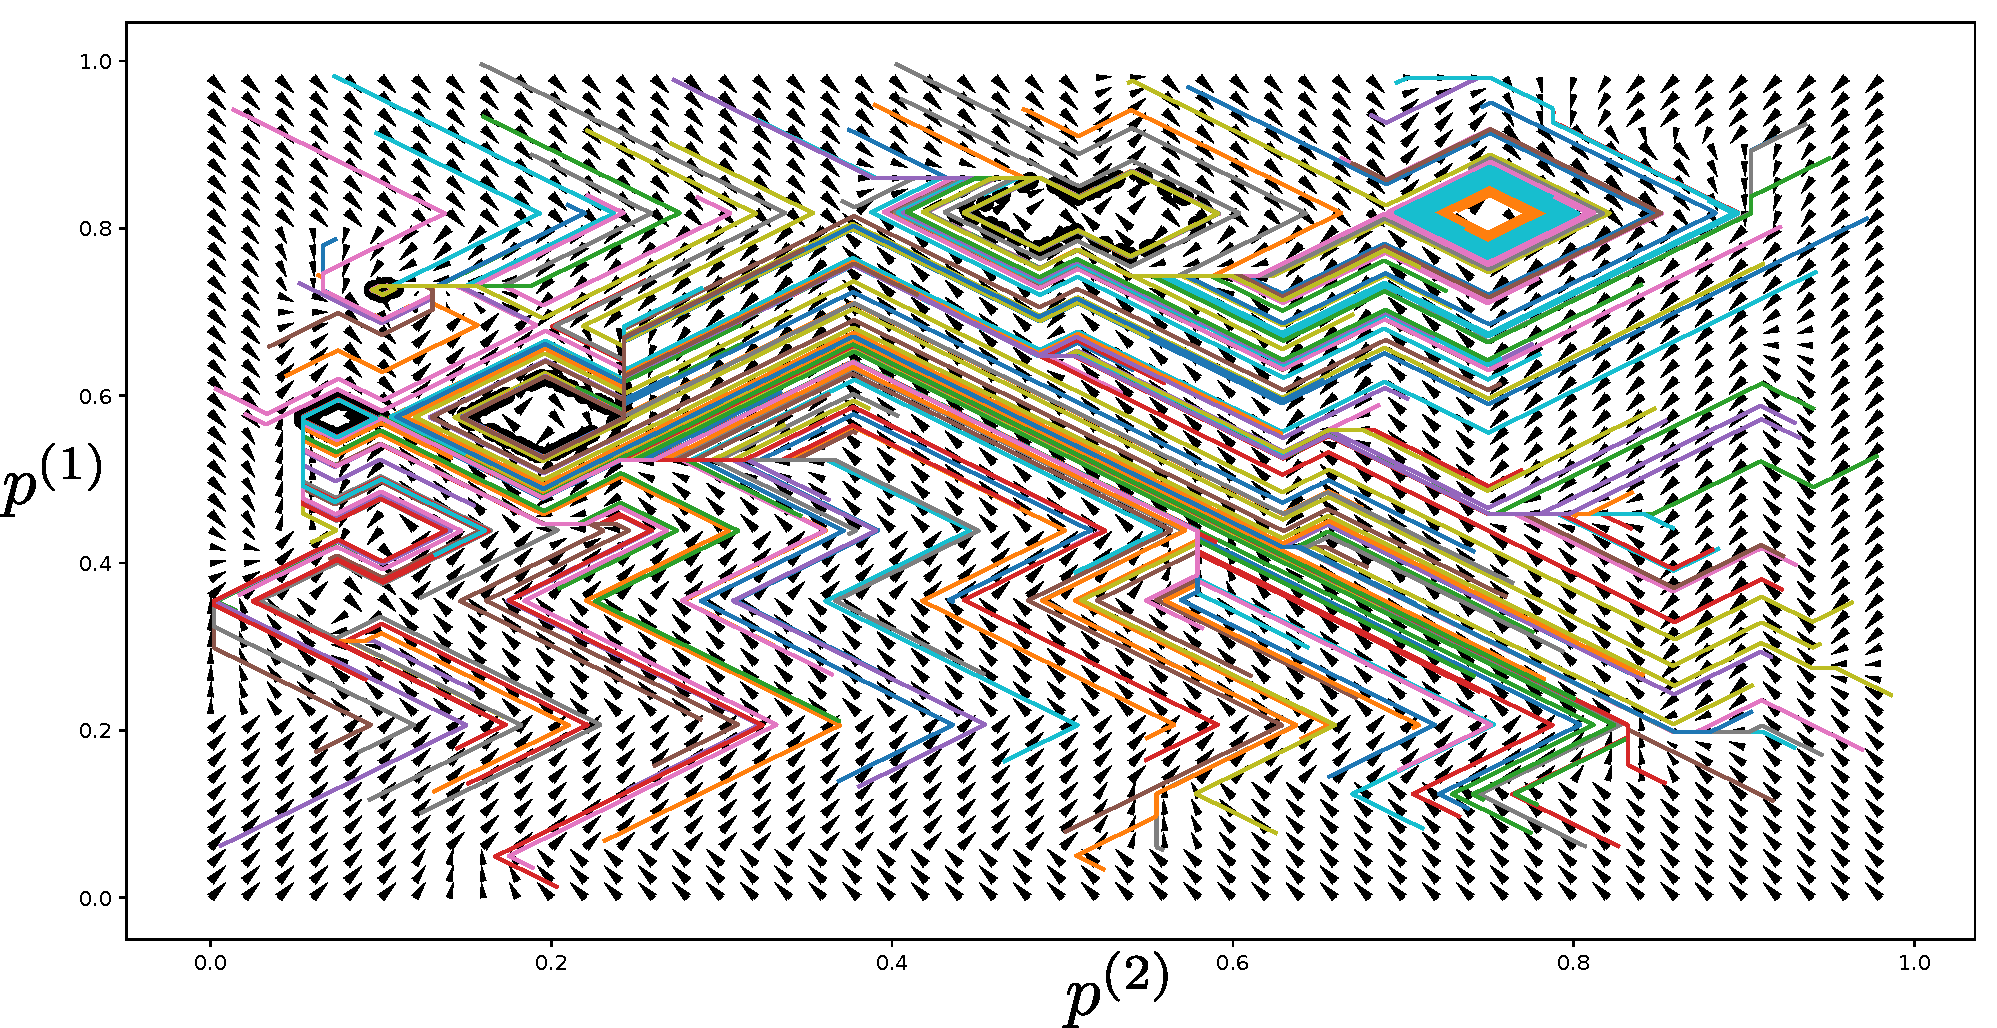
\includegraphics[width=\textwidth]{champ_006_t1.pdf}
\caption{Champ de déplacements de $\bmu\m{1},\bmu\m{2}$ lorsque les poids sont encore aléatoires, à $t=0$. Les trajectoires de 200 relaxations, initialisées différemment, sont représentées. En fonction de la position initiale des BMUs, la relaxation évolue vers un point fixe ou un cycle limite. }
\label{fig:champ_0}
\end{figure}


\begin{figure}
\centering
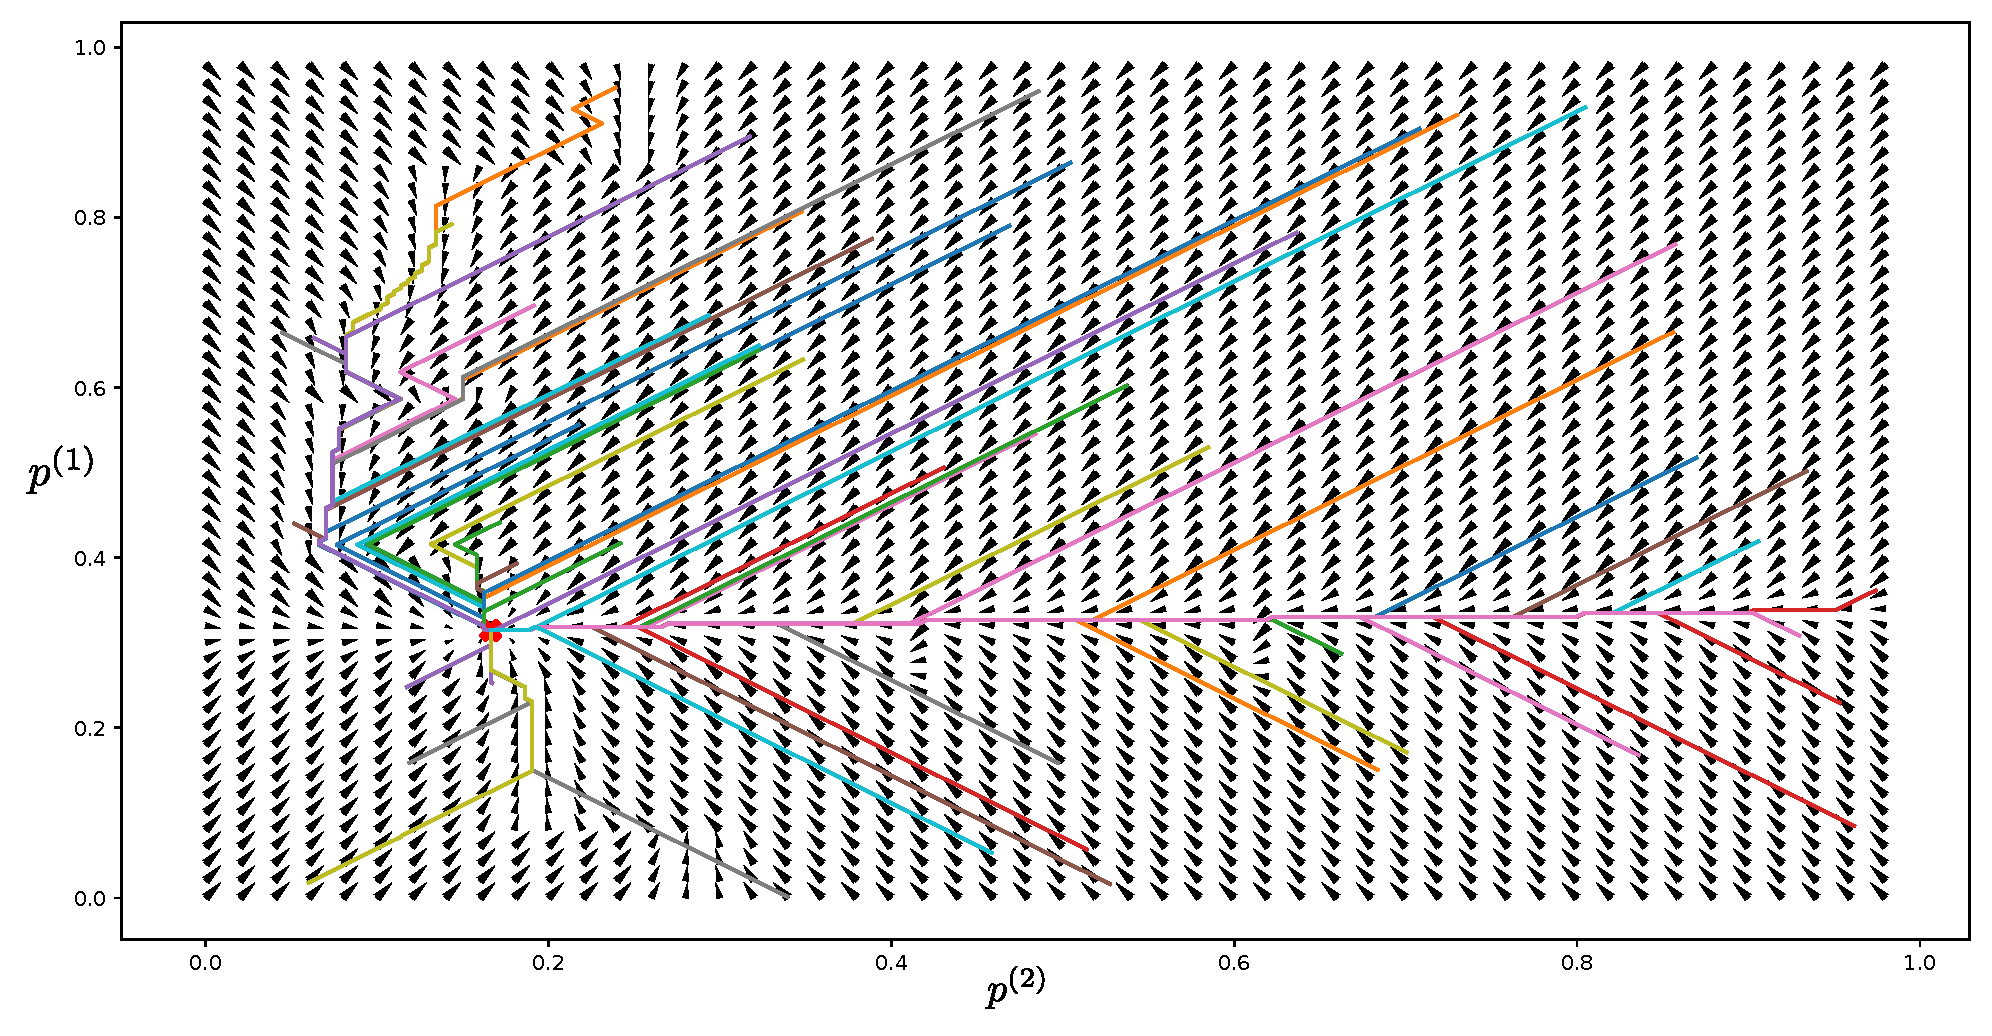
\includegraphics[width=\textwidth]{champ_006.pdf}
\caption{Champ de déplacements de $\bmu\m{1},\bmu\m{2}$ lorsque les poids sont organisés tels que représentés en figure \ref{fig:w006}, à $t=9999$.es trajectoires de 50  relaxations, initialisées différemment, sont représentées. Les relaxations évoluent vers un point fixe commun.}
\label{fig:champ_9999}
\end{figure}

\subsection{Influence du pas de relaxation}

Dans les expériences précédentes, on a utilisé un pas de convergence $\delta=0.05$. Une autre solution est de ne pas utiliser de pas de relaxation, c'est à dire, à chaque itération, déplacer le BMU $\bmu\m{i}$ directement à la position ou l'activité globale est maximale, au lieu de le déplacer de $\delta$ vers cette position.
L'évolution de la relaxation devient alors:
\begin{equation}
\forall i, \bmu\m{i}_{\tau+1} = \hat{p}\m{i}_{\tau}
\end{equation}
En figure \ref{fig:diff_nopas}, on trace différentes trajectoires de relaxation, pour une même entrée. Ces relaxation sont effectués après l'apprentissage des données par l'architecture. Le processus de relaxation effectué pendant l'apprentissage n'utilise pas de déplacement $\delta$ non plus. 
On représente sur cette même figure les différences ${\hat{p}}\m{1} - p\m{1}$ et ${\hat{p}}\m{2} - p\m{2}$. La relaxation semble encore converger vers un point fixe.


\begin{figure}
\begin{minipage}{0.5\textwidth}
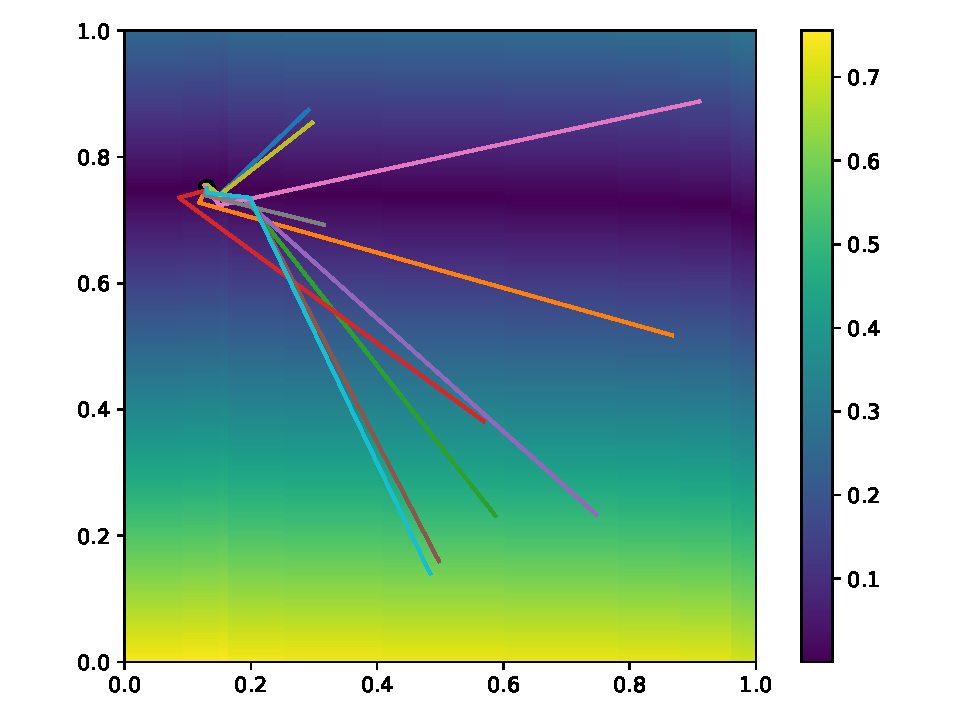
\includegraphics[width=\textwidth]{champ_X_009}
\end{minipage}
\begin{minipage}{0.5\textwidth}
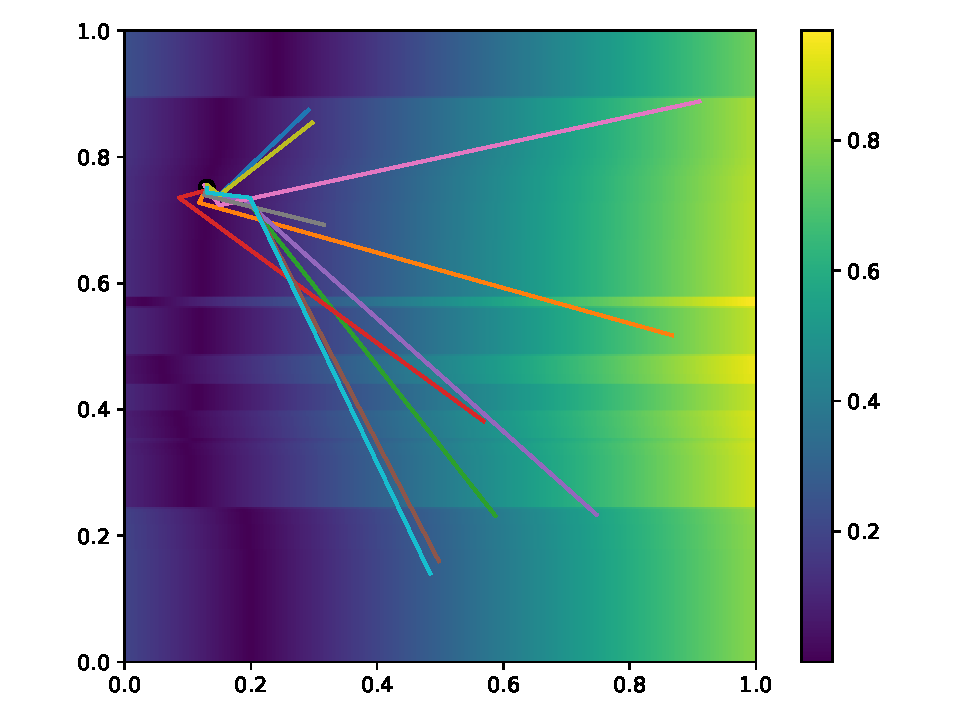
\includegraphics[width=\textwidth]{champ_Y_009}
\end{minipage}
\caption{Trajectoires des relaxations $(\bmu\m{1}_{\tau},\bmu\m{2}_\tau)$ dans le champ des différences ${\hat{p}}\m{1} - p\m{1}$ et ${\hat{p}}\m{2} - p\m{2}$, lorsque la relaxation est effectuée sans utiliser de petits déplacements. Les tracés sont effectués après apprentissage. La relaxation semble encore converger vers un point fixe.}
\label{fig:diff_nopas}
\end{figure}

\section{Discussion}

Les parties \ref{sec:conv} et \ref{sec:cont} montrent que, lorsque les poids sont quelconques, la convergence de l'algorithme de relaxation n'est pas assurée; au contraire, la relaxation évolue dans la plupart des cas vers une situation non convergente. Dans le cas particulier étudié dans la section, il semble exister des point fixes, mais dus au caractère aléatoire des poids. La relaxation ne permet pas de trouver ces points. Pourtant, l'apprentissage des cartes utilisant la relaxation comme recherche de BMU mène une organisation des poids, même sans que la relaxation ne converge au début. Cette organisation permet de plus une meilleure convergence de la relaxation (convergence dans plus de $90 \%$ des cas).

Ce comportement peut être expliqué. On observe que la relaxation converge bien à partir du moment où les poids externes sont organisés et présentent une continuité. Au début de l'apprentissage, même si la relaxation mène à des positions quelconques de BMUs, ces BMUs auront quand même des poids externes proches de la valeur de l'entrée. Le calcul de l'activité dépend en effet d'abord de l'activité externe de la carte:
$$ a_g = \sqrt{a_e ( \beta a_e + (1-\beta a_c))}, \;\; \beta=0.5$$ 
De plus, la relaxation est initialisée à une position correspondant au maximum de l'activité externe.
L'organisation de la carte s'effectuera donc de façon similaire à une carte classique. Dans une carte de Kohonen, pour des poids aléatoires, de multiples positions de BMU sont possibles lors du calcul de la distance des poids à l'entrée. La disposition des poids et le choix du BMU n'influencent pas la propriété globale d'organisation d'une carte. Cette même observation peut s'effectuer ici. 
Le rayon de voisinage externe étant bien plus grand que le rayon de voisinage contextuel, l'organisation des poids externes de la carte influence peu l'organisation des poids contextuels.
Lorsque les poids externes présentent une continuité, la relaxation converge. Les poids contextuels peuvent alors s'organiser selon le BMU, qui a maintenant un sens: il s'agit d'un point fixe de la fonction de relaxation. Le BMU correspond alors au point qui maximise en même temps les activités globale de chaque carte.

Expérimentalement, on observe que, lorsque les cartes sont organisés, le point fixe est atteint par n'importe quelle trajectoire de relaxation. Le BMU a donc un sens au niveau de la carte. 

Enfin, la relaxation dépend du pas de déplacement utilisé $\delta$. On pourrait supposer que prendre un petit $\delta$ permet une meilleure convergence; en fait, la valeur de $\delta$ influence peu la capacité de convergence et l'organisation des cartes. La relaxation pourrait être effectuée sans utiliser de pas de relaxation. Par ailleurs, la relaxation est initialisée proche de la position théorique du BMU, quand elle existe. La relaxation est donc finalement assez courte.


\section{Etude de l'influence de l'entrée contextuelle sur le BMU}\label{sec:cont}

Dans cette section, nous étudions plus précisément l'évolution de la suite $(\mathbf{\bmu})_{\tau}$ dans le cas de d'une architecture de deux cartes 1D connectées. Les cartes sont $M\m{1}$ et $M\m{2}$ prenant en entrée externe respectivement $\inpx\m{1} = X, \inpx\m{2} = Y$, coordonnées des points d'un cercle 2D.
Les entrées contextuelles des deux cartes sont à valeurs dans l'espace des positions d'une carte: $\inpc\m{1} = \bmu\m{2}$ et $\inpc\m{2} = \bmu\m{1}$.
On définit les valeurs $\hat{p}\m{1}$ et $\hat{p}\m{2}$ comme indiqué dans l'équation \ref{eq:pstar}
\begin{equation} 
\begin{cases}
	\hat{p}\m{1}_{\tau} = \argmax_{p\m{1}}(a_g(p\m{1},\bmu\m{2}_{\tau})) \\
	\hat{p}\m{2}_{\tau} = \argmax_{p\m{2}}(a_g(p\m{2},\bmu\m{1}_{\tau})) \\
\end{cases}
\end{equation}

Nous tracons ensuite les valeurs de $\hat{p}\m{1}$ en fonction de son entrée contextuelle $\bmu\m{2} \in [0,1]$, et $\hat{p}\m{2}$ en fonction de $\bmu\m{1} \in [0,1]$ en figure \ref{fig:w006}.
Cette expérience est réalisée après l'apprentissage. On remarque que, $\hat{p}\m{i}$ varie peu en fonction de l'entrée contextuelle de la carte; tout le processus de relaxation se déroulera donc dans une portion réduite de la carte. Cette propriété favorise la convergence de la relaxation.
En réalisant les mêmes tracés à des étapes différentes de l'apprentissage, on peut faire l'hypothèse que la dépendance de $\hat{p}$ à l'entrée contextuelle dépend surtout de l'organisation des poids externes. En effet, l'activité externe est prépondérante dans le calcul de l'activité globale. Les poids externes s'organisent plus rapidement que les poids contextuels dus à la différence de rayons de voisinage. A partir du moment ou les poids externes d'une carte $i$ sont dépliés, les valeurs possible pour $\bmu\m{i}$ restent dans une portion limitée de la carte. Cela permet alors à la relaxation de trouver un point fixe dans cette portion.

\begin{figure}
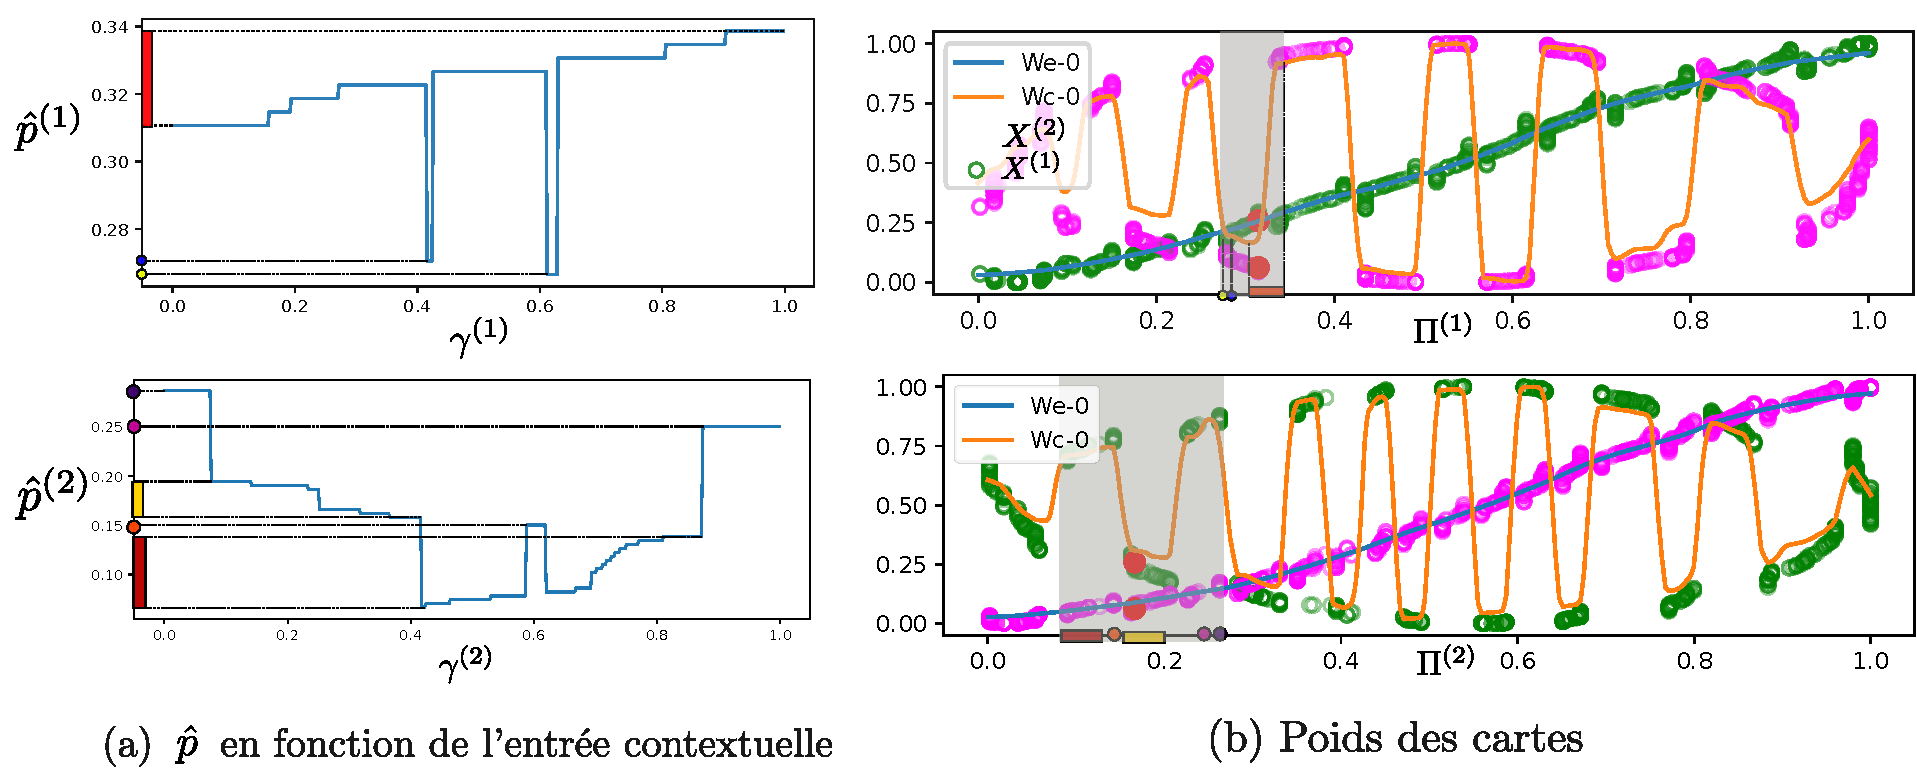
\includegraphics[width=\textwidth]{am_w_006}
\caption{(a): $\hat{p}\m{1}$ et $\hat{p}\m{2}$ en fonction de l'entrée contextuelle de leur carte $\bmu\m{2}$ et $\bmu\m{1}$.(b): les poids externes et contextuels des cartes $1$ et $2$ sont représentés selon leur position dans la carte. On représente également les entrées test $\inpx\m{1}$ et $\inpx\m{2}$ en fonction de leur BMU. Les entrées utilisées pour tracer les figures de gauche sont colorées en rouge sur les figure de droite: $\inpx\m{1}=0.26,\inpx\m{2}=0.06$. Les intervalles dans lequel les valeurs de $\hat{p}$ varient sont reportés sur la figure (b).}
\label{fig:w006}
\end{figure}

\subsection{Conclusion}
La relaxation est donc une recherche d'un maximum global à l'architecture, ce maximum étant un point fixe de la fonction de mise à jour des positions.
Une fois que les poids externes d'une carte présentent une continuité, la relaxation et le BMU issu de ce processus ont un sens topologique: on observe expérimentalement que la fonction de mise à jour présente un point fixe $\mathbf{\bmu} = \mathbf{f}(\mathbf{\bmu})$, et que la relaxation converge vers ce point fixe. Ce point fixe est alors le point qui maximise \emph{collectivement} les activités globales de chaque carte de l'architecture.
Bien que la relaxation ne converge pas au début de l'apprentissage, la convergence est observée dès que les poids externes présentent une certaine continuité. Cette continuité étant assurée après quelques itérations d'apprentissage par l'algorithme de mise à jours des poids de Kohonen, on peut donc dire que la relaxation converge au sein de CxSOM. Cette convergence est observée pour des cartes en une et deux dimensions.
La relaxation est alors un moyen de trouver un ensemble de BMU au sein d'une architecture maximisant une propriété \emph{globale} à cette architecture: toutes les cartes voient leur activité globale maximisée. Les BMUs ont donc un sens topologique. Cette recherche de maximum est réalisée localement, au niveau de chaque carte, et non de façon globale. La relaxation agit alors comme une manière de connecter des cartes de façon non-hiérarchique, avec un calcul décentralisé.

\ifSubfilesClassLoaded{
    \printbibliography
    %\externaldocument{../main.tex}   
}{}
\end{document}
